\section{Classification}
\thispagestyle{plain}

As in regression, we are in the land of supervised learning. However,
here our labeling is a category, $\mathcal{D} = \{ \vec{x}_i, c_i \}$,
where $c_i \in \{1, 2, \ldots, C\}$, and $C$ is the number of classes.

\bluebox{\textbf{Aim:} Given a new $\vec{x}$, we want to predict its class.}

Regions where certain classes are predicted are separated by
decision boundaries. An example classification is shown in
figure \ref{fig:classification}.

\begin{figure}[H]
  \centering
  \includesvg[width=0.5\textwidth]{figures/classification.svg}
  \caption{Example classification.}
  \label{fig:classification}
\end{figure}

\subsection{Overview on approaches to classification}
In the Bayesian perspective
\begin{itemize}
    \item we model the likelihood of data given the class and from Bayes theorem we can make predictions on class label probabilities $\rightarrow$ \textbf{Bayesian classifiers}, e.g. Naive Bayes, etc.
\end{itemize}
where
\begin{itemize}
    \item modeling the likelihoods of data given class with a simple Gaussian distribution gets us to \textbf{discriminant analysis} (\textit{data modeling culture})
\end{itemize}

More belonging to the \textit{algorithmic culture}, we can
\begin{itemize}
    \item assign a label to a new point based on a majority vote of its $k$ nearest neighbors $\rightarrow$ \textbf{k-NN}
    \item partition feature space by recursive binary splits in a tree-structure, devising a partitioning where each region is assigned a class $\rightarrow$ \textbf{decision trees}
    \item use multiple of such trees e.g. trained on bootstrap samples of the data and e.g. majority vote for a decision $\rightarrow$ \textbf{random forests}
\end{itemize}

In the special case of two classes, we can
\begin{itemize}
    \item find the linear border between the classes (if possible) minimizing the closest distance to any point of the classes $\rightarrow$ \textbf{support vector machines}
    \item use a GLM for a Bernoulli distribution, so directly model the likelihood of class labels given a probability
    model which mean is modeled depending on the features $\rightarrow$ \textbf{logistic regression}
\end{itemize}

Multiple classes can e.g. be modeled by $K$ 1-vs-all classifications for $K$ classes,
where each classifier is trained to distinguish one class from all other $K-1$ classes.

\greenbox{Logistic regression can also easily be extended to multiple classes by using a softmax function,
to model the class probabilities, which are the parameters of a multinomial distribution,
describing the likelihood of the observed class labels given the data.}

\subsection{Discriminant analysis}
Discriminant analysis is a Bayesian classifier where the class of a new data point is given by
\begin{equation}
    k^* = \argmax_k p(c = k | \vec{x})
\end{equation}
In discriminant analysis, the likelihood of the data given a class is modeled by a Gaussian whose mean
and covariance are estimated from the training data which is of that class.
\begin{equation}
    \begin{aligned}
        p(\vec{x}_i | c_i = k) &= \mathcal{N}(\vec{\mu}_k, \mat{\Sigma}_k) \\
                               &= (2\pi)^{-\frac{p}{2}} (\det \mat{\Sigma}_k)^{-\frac{1}{2}} \exp \left( -\frac{1}{2} (\vec{x}_i - \vec{\mu}_k)^T \mat{\Sigma}_k^{-1} (\vec{x}_i - \vec{\mu}_k) \right)
    \end{aligned}
\end{equation}
Applying Bayes' theorem yields

\begin{equation}
    p\left(k \mid \vec{x}_i\right)=\frac{p\left(\vec{x}_i \mid k\right) p(k)}{\sum_{l=1}^K p\left(\vec{x}_i \mid l\right) p(l)}, \quad p(l)=\frac{\# \text { data points of class } l}{\# \text { all data points in training set }}
\end{equation}

In figure \ref{fig:discriminant_analysis}, we see an example of discriminant analysis in 1D.

\begin{figure}

    \centering
    \begin{subfigure}{0.55\textwidth}
      \centering
      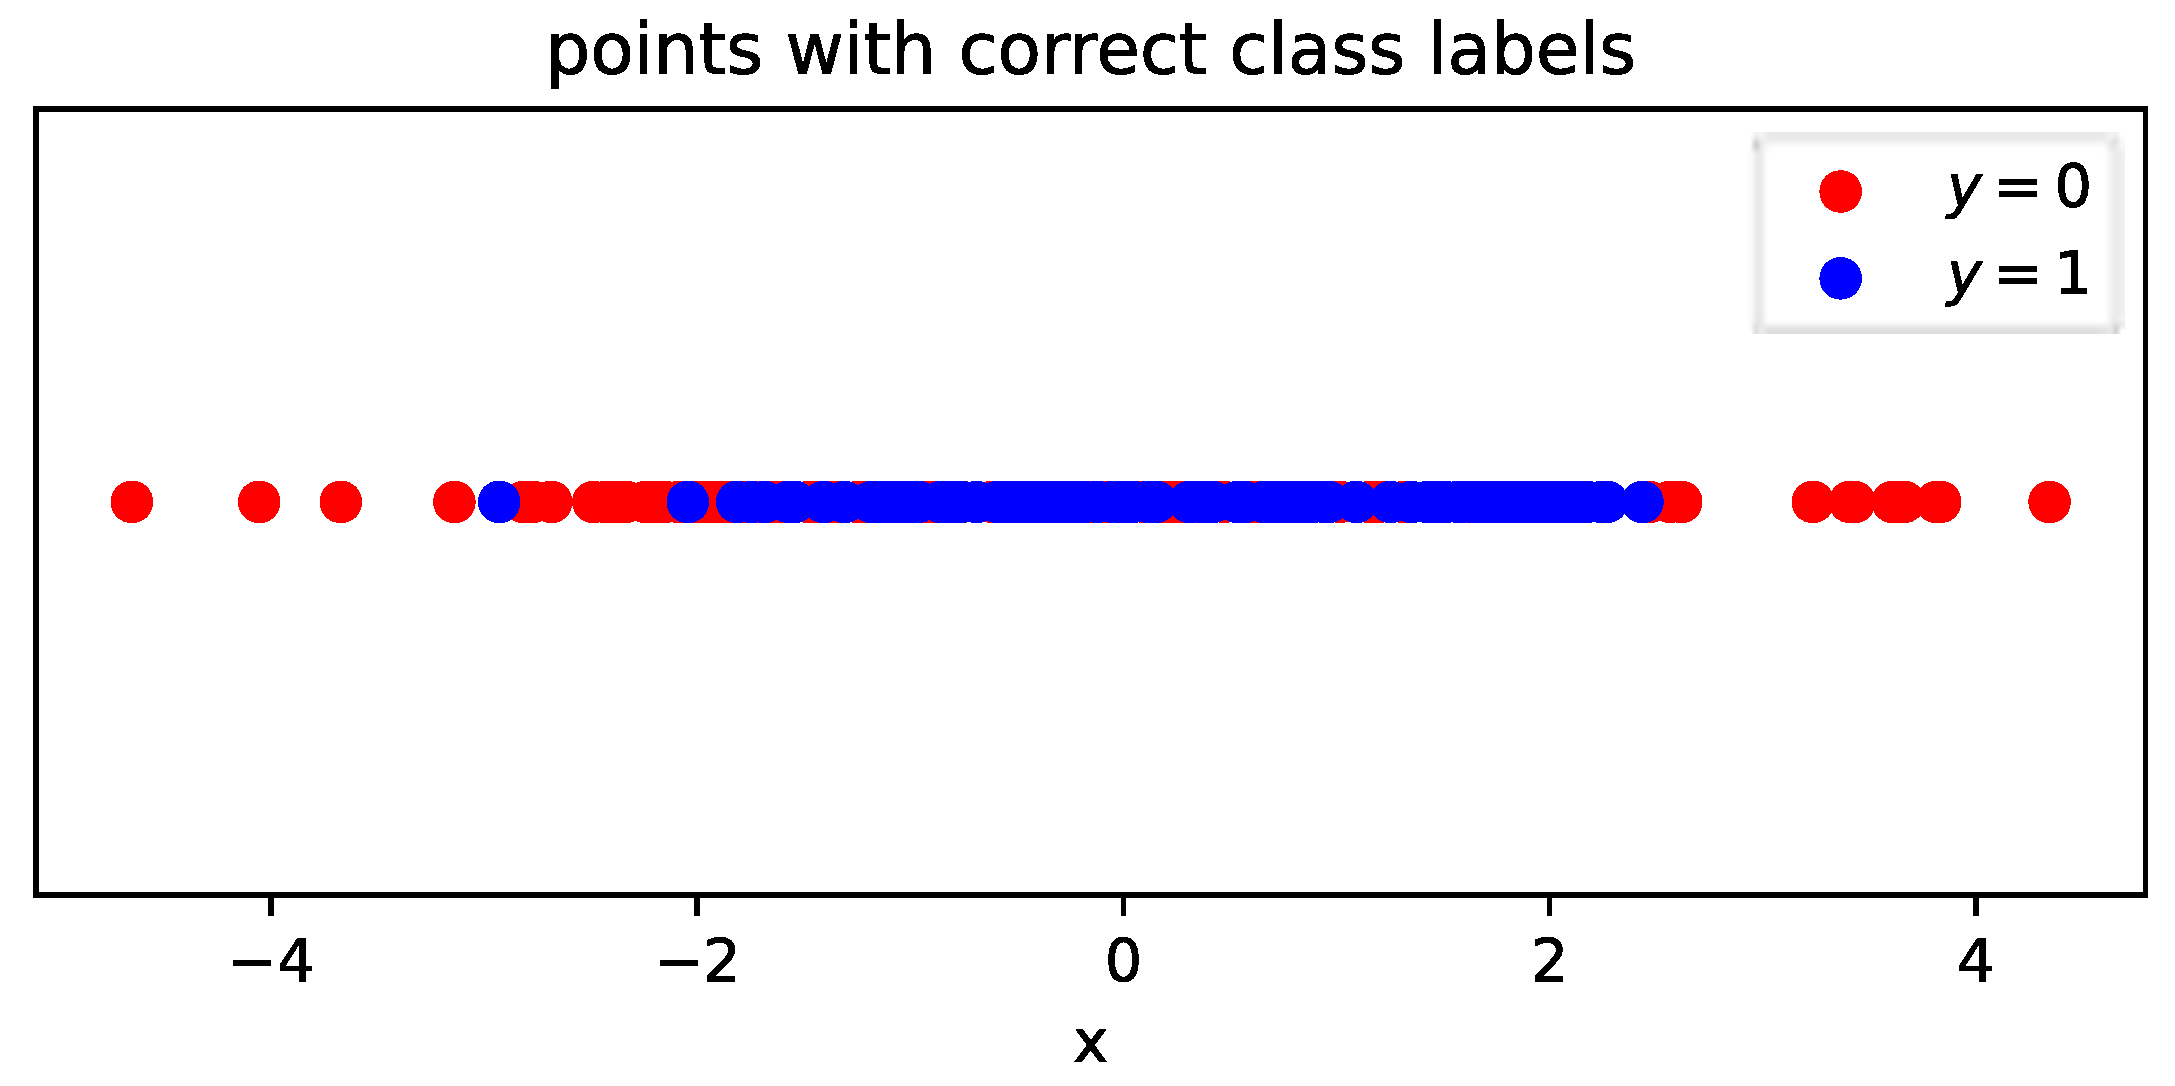
\includegraphics[width=.95\linewidth]{figures/dist.pdf}
      \caption{Given data. For instance the weights of examplares of African Forest Elephants (red) and Asian Elephants (blue), for which a Gaussian distribution
      seems reasonable.}
      \label{fig:discriminant_analysis_data}
    \end{subfigure}%



    \begin{subfigure}{0.55\textwidth}
      \centering
      \includesvg[width=.95\linewidth]{figures/class_fits.svg}
      \caption{Fits of the class probability densities. So really just a Gaussian density fit to the African and Asian elephant measurements respectively.}
      \label{fig:discriminant_analysis_fits}
    \end{subfigure}



    \begin{subfigure}{0.55\textwidth}
        \centering
        \includesvg[width=.95\linewidth]{figures/posteriors.svg}
        \caption{Posteriors, as the read class has higher spread, outer points are assigned to it. Given the weight, what kind of elephant do we assume?
        As the forest elephant comes in a wider range of weights, at the extremes we assume forest elephant.}
        \label{fig:discriminant_analysis_posteriors}
      \end{subfigure}

    \caption{Example of discriminant analysis in 1D.}
    \label{fig:discriminant_analysis}

\end{figure}

\subsubsection{Linear discriminant analysis (LDA) and Mahalanobis distance}
\bluebox{\textbf{Assumption of LDA:} We assume all classes to share a common covariance 
matrix $\mat{\Sigma}_k = \mat{\Sigma}$ (also leading to a more robust estimation of $\mat{\Sigma}$).}

\textcolor{blue1}{Discriminant function:} For assigning a class, we only need to know
which posterior is larger, not the absolute value, so we can equivalently consider
the discriminant function (as always the evidence term $p(\vec{x})$ is the same for all classes,
and we apply the strictly monotonic $\log$ function):

\begin{equation}
    \begin{aligned}
    \delta_k\left(\vec{x}_i\right)&:=\ln \left(\exp \left(-\frac{1}{2}\left(\vec{x}_i-\vec{\mu}_k\right)^T \mat{\Sigma}^{-1}\left(\vec{x}_i-\vec{\mu}_k\right)\right) p(k)\right) \\
    &=-\textcolor{pink1}{\frac{1}{2}\left(\vec{x}_i-\vec{\mu}_k\right)^T \mat{\Sigma}^{-1}\left(\vec{x}_i-\vec{\mu}_k\right)}+\ln (p(k)) \\
    &=-\textcolor{pink1}{D_{\text {mah }}^2}+\ln (p(k))
    \end{aligned}
\end{equation}

with the decision criterion

\begin{equation}
    \hat{k} = \argmax_k p(c = k|\vec{x}_i) = \argmax_k{\delta_k\left(\vec{x}_i\right)}
\end{equation}

which is the \textcolor{green1}{Bayes optimal classifier} if our assumtion $\sim \mathcal{N}(\vec{\mu}_k, \mat{\Sigma})$ is valid.

\pinkbox{\textbf{Mahalanobis distance:} $D_\text{mah}$ measures the distance of a measurement $\vec{x}_i$ to the class mean $\vec{\mu}_k$ normalized
by the covariance matrix $\mat{\Sigma}$. The Mahalanobis distance to a class with high spread might be smaller than
to a class with low spread, even if the Euclidean distance to the mean of the class with high spread is larger,
see figure \ref{fig:mahalanobis}. This is not the case in LDA though, as $\mat{\Sigma}_k = \mat{\Sigma}$ is assumed.}

\begin{figure}[!htb]
    \centering
    \includesvg[width=0.8\textwidth]{figures/mahalanobis.svg}
    \caption{Mahalanobis distance.}
    \label{fig:mahalanobis}
\end{figure}

\yellowbox{\textbf{Sidenote on multivariate hypothesis testing:} By the t-test we can test if
given data supports the hypothesis that a mean is of a certain value or means of two samples (or classes) are equal \textbf{in the
univariate case}. The multivariate analogue of the one-sample t-test is the \textbf{Hotelling's T-squared test} and the
test statistic $t^2 = D_{\text{mah}}^2 \sim T^2_{p,N-1} = \frac{p(N-1)}{N-p} F_{p,N-p}$, where $p$ is the number of dimensions,
$N$ the number of data points, and $F_{p,N-p}$ the F-distribution. For $\mat{\Sigma}$ the sample covariance
\begin{equation}
    \mat{\hat{\Sigma}} = \frac{1}{N-1} \sum_{i=1}^N (\vec{x}_i - \vec{\mu})(\vec{x}_i - \vec{\mu})^T
\end{equation}
is used. An analogue two-sample test, to compare if two classes have the same mean in the multivariate case, is 
done with a pooled covariance matrix.}

\subsubsubsection{The LDA decision surface is linear}
The decision surface between class $k$ and $l$ is given by
\begin{equation}
    \delta_k\left(\vec{x}\right) = \delta_l\left(\vec{x}\right)
\end{equation}
so given by
\begin{equation}
    \log \frac{p(k)}{p(l)} - \frac{1}{2} \left( \vec{x} - \vec{\mu}_k \right)^T \mat{\Sigma}_k^{-1} \left( \vec{x} - \vec{\mu}_k \right) + \frac{1}{2} \left( \vec{x} - \vec{\mu}_l \right)^T \mat{\Sigma}_l^{-1} \left( \vec{x} - \vec{\mu}_l \right) = 0
\end{equation}
where for LDA, so $\mat{\Sigma}_k = \mat{\Sigma}_l = \mat{\Sigma}$, the quadratic terms cancel,
and we are left with a linear decision boundary.

\bluebox{\textbf{Quadratic discriminant analysis (QDA):} Not assuming the same covariance matrices, we get quadratic decision boundaries in $\vec{x}$, so
ellipses, hyperboloids, parabolas, parallel lines. An example for QDA is shown in figure \ref{fig:qda}.}

\begin{figure}[!htb]
    \centering
    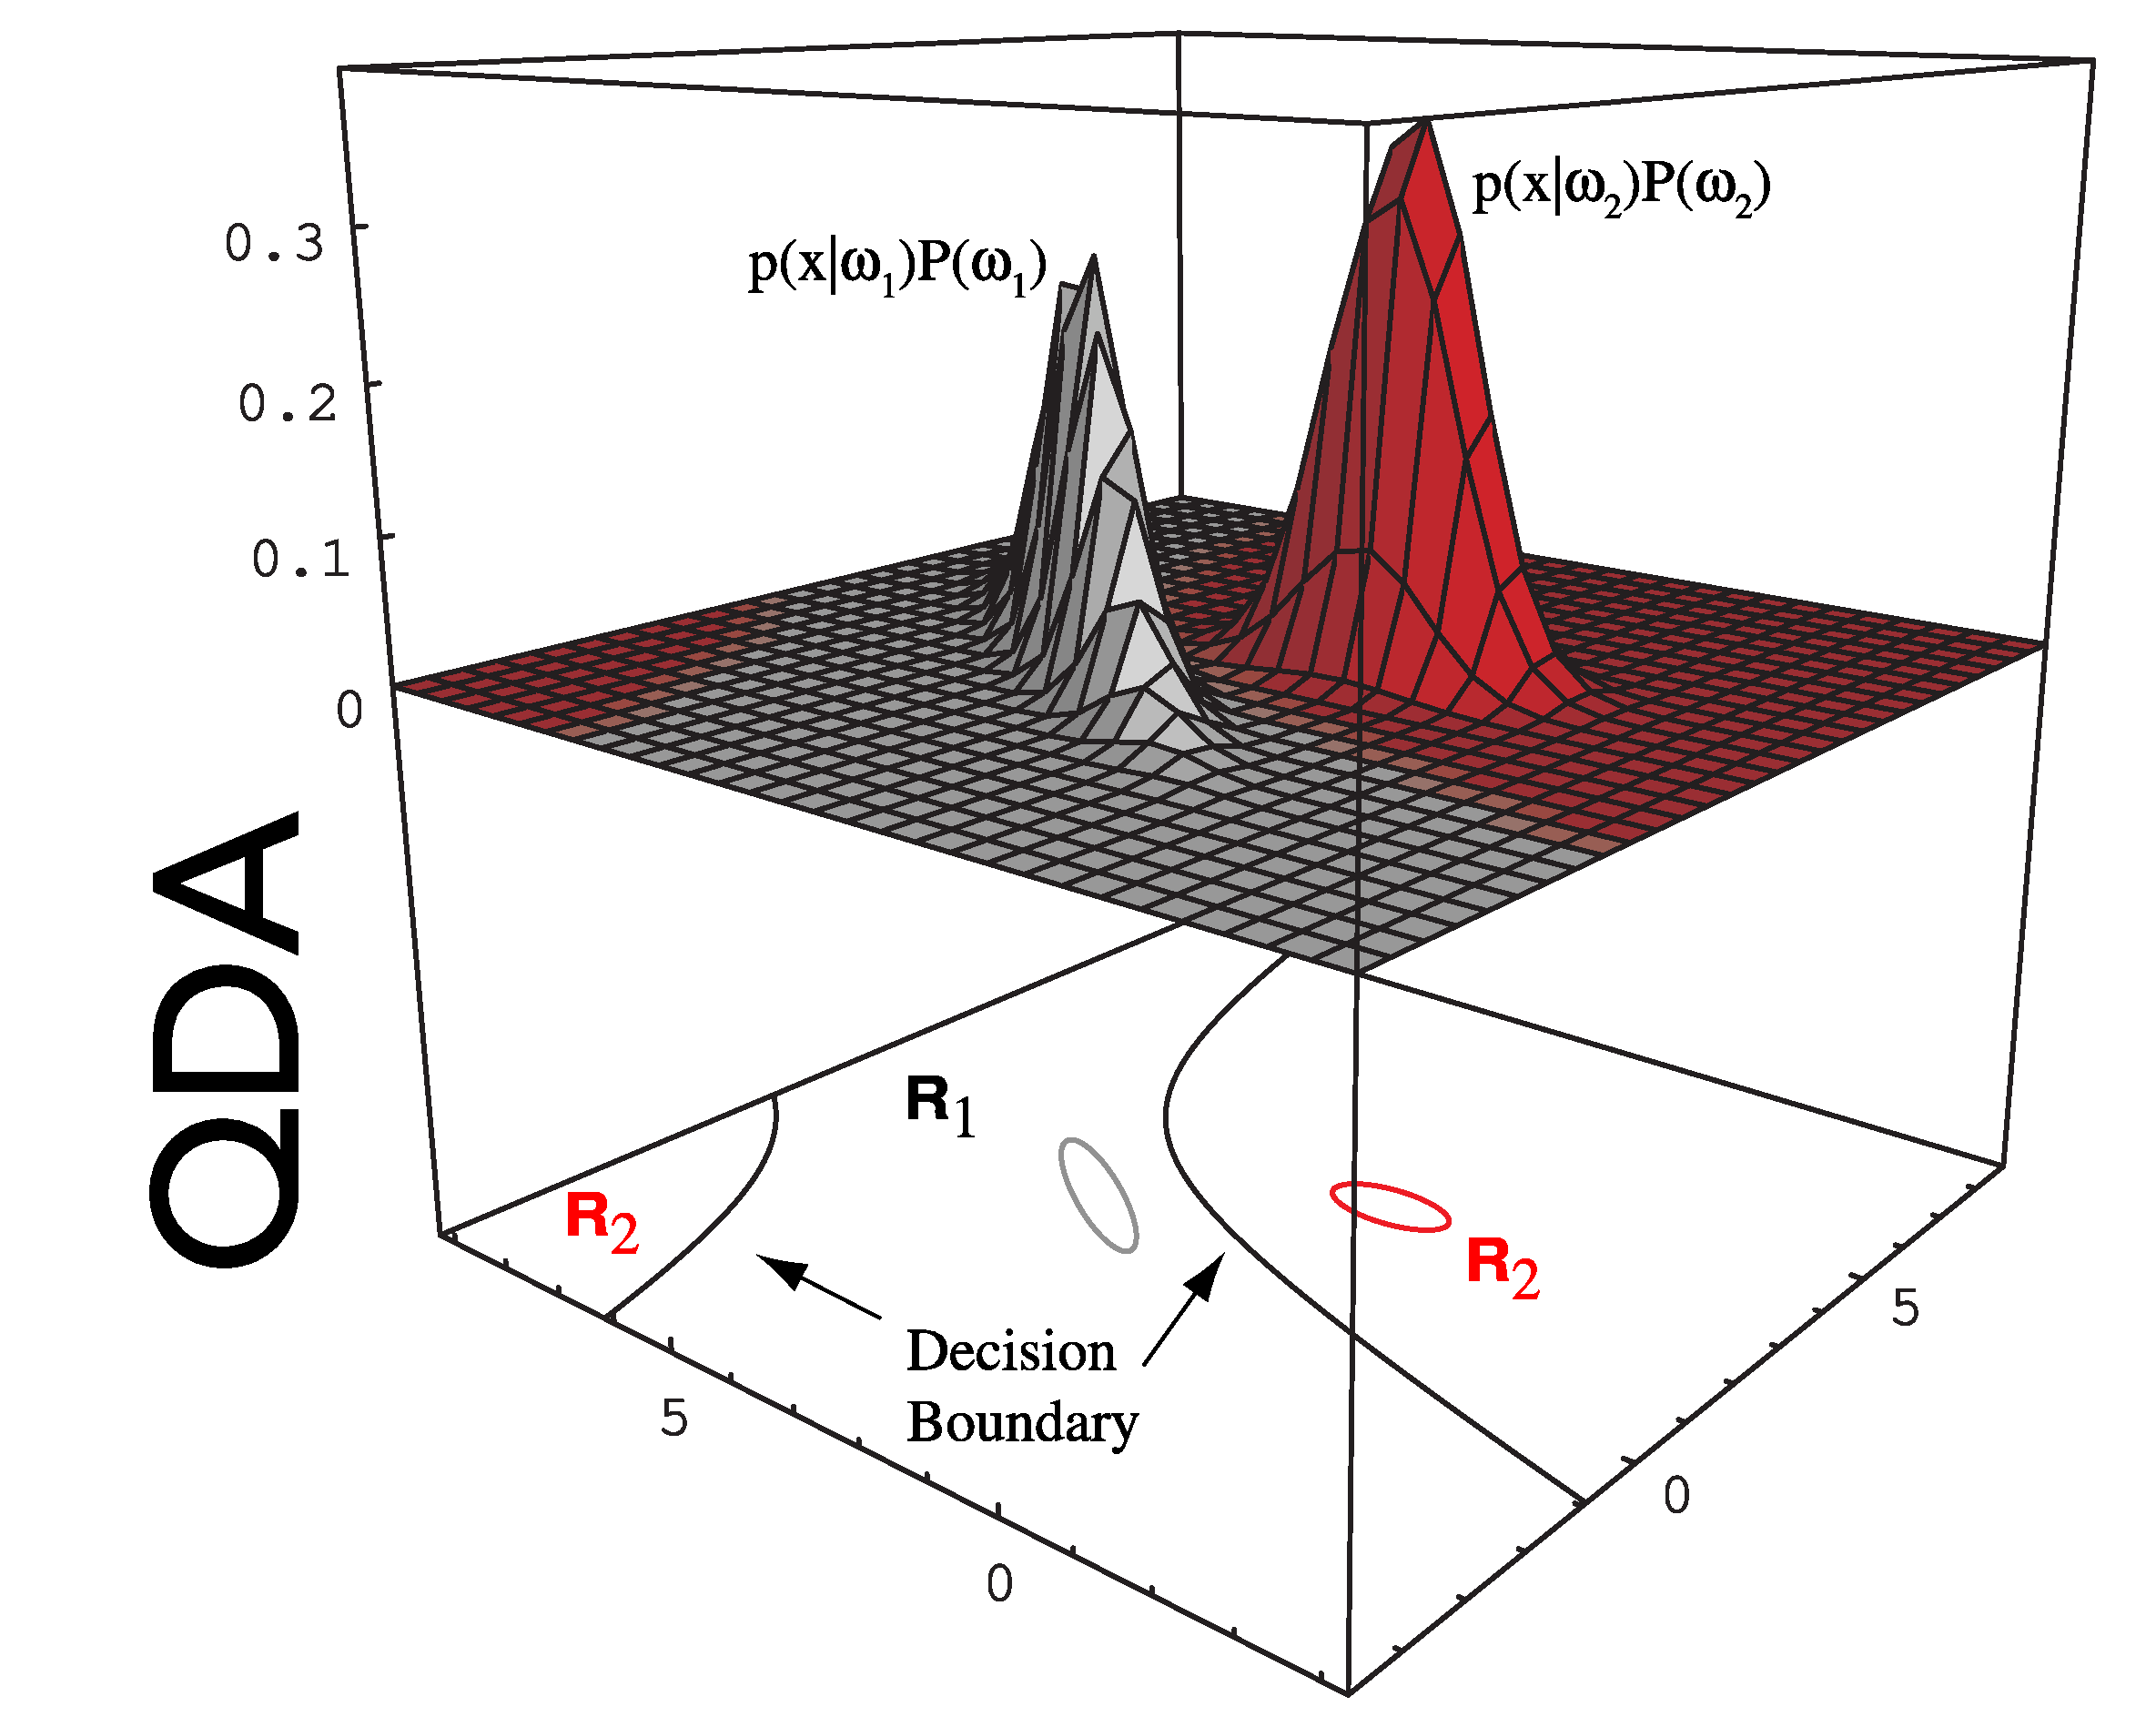
\includegraphics[width=0.6\textwidth]{figures/qda.pdf}
    \caption{Example of QDA. Class likelihoods in red and grey, decision boundaries drawn below.}
    \label{fig:qda}
\end{figure}

\subsubsection{Estimation of the prior, mean and covariance in discriminant analysis}
The \textcolor{blue1}{prior} is estimated by class proportions in the training data as

\begin{equation}
    \hat{p}\left(c_i=k\right)=\frac{\# \text { data points of class } k}{\# \text { all data points in training set }}=\frac{N_k}{N}, \quad N=\sum_{l=1}^K N_l
\end{equation}

the \textcolor{blue1}{class means} intuitively by

\begin{equation}
    \vec{\hat{\mu}}_k=\frac{1}{N_k} \sum_{\vec{x}_i \text { for } c_i=k} \vec{x}_i, \quad \vec{x}_i \in \mathbb{R}^p
\end{equation}

and the \textcolor{blue1}{class covariances} by

\begin{equation}
    \mat{\hat{\Sigma}}_k=\frac{1}{N_k-1}\left(\mat{X}_{(k)}-\underset{N_k \times 1}{\vec{1}} \vec{\hat{\mu}}^T\right)^T\left(\mat{X}_{(k)}-\underset{N_k \times 1}{\vec{1}} \vec{\hat{\mu}}^T\right)
\end{equation}

where in LDA, we use the pooled covariance matrix

\begin{equation}
    \mat{\hat{\Sigma}}=\frac{1}{N-K}\sum_{k=1}^K \left(N_k-1\right) \mat{\hat{\Sigma}}_k
\end{equation}

\subsubsubsection{Advantages of Discriminant Analysis}
While Gaussian class likelihoods are a strong assumption
\begin{itemize}
    \item Discriminant analysis is very robust, no hyperparameters to tune
    \item and Gaussian class probabilities are common by the central limit theorem
\end{itemize}

\subsection{Linear Classifiers}
A linear decision boundary (or hyperplane) can generally be
given by its normal vector $\vec{w}$ and an offset $b$ as
\begin{equation}
    g(\vec{x}) = \vec{w}^T \vec{x} - b
\end{equation}
(we will sometimes use $\vec{\beta} = \vec{w}$ and $\beta_0 = -b$).
The \textbf{decision} on what class to assign to a point $\vec{x}$ is given
by the sign of $g(\vec{x})$. For instance
\begin{itemize}
    \item in Support Vector Machines, we have class labels $y_i \in \{-1, 1\}$, so $\hat{c}_i = \sign(g(\vec{x}_i))$, a sign-classifier is illustrated in figure \ref{fig:sign_classifier}
    \item in logistic regression, we model the probability of class $1$, $p(c = 1 | \vec{x}) = \sigma(g(\vec{x}))$, so $p(c = 0 | \vec{x}) = 1 - \sigma(g(\vec{x}))$
\end{itemize}
The decision boundary is given by
\begin{equation}
    \vec{x} \text{ on boundary}: g(\vec{x}) = 0
\end{equation}

\bluebox{In each case, our aim is to find the in some sense best $\vec{w}$ and $b$, specifying the separating hyperplane and decision function.}

\begin{figure}[!htb]
    \centering
    \includesvg[width=0.6\textwidth]{figures/sign_classifier.svg}
    \caption{Sign classifier.}
    \label{fig:sign_classifier}
\end{figure}

\subsection{Support Vector Machines (SVM)}
An SVM is a non-probabilistic binary classifier with linear decision boundary. Given
a training set $\mathcal{D} = \{ \vec{x}_i, c_i \}$, $c_i \in \{-1, 1\}$, we want
to assign a class to a new point $\vec{x}$.

\subsubsection{Basic Idea of SVMs - maximum margin classifier}
We are using a liner classifier
\begin{equation}
    g(\vec{x}) = \vec{\beta}^T \vec{x} + \beta_0
\end{equation}
with sign decision function
\begin{equation}
    \hat{c} = \sign(g(\vec{x}))
\end{equation}
\bluebox{What seperating hyperplane is best?}
Consider the example of two linearly separable classes in figure \ref{fig:svm_simple}. In the figure
$H_1$ does not event separate the classes - $H_2$ and $H_3$ both do is perfectly. So why is
$H_3$ the better choice?

\begin{figure}[!htb]
    \centering
    \includesvg[width=0.6\textwidth]{figures/svm_simple.svg}
    \caption{Example of two linearly separable classes.}
    \label{fig:svm_simple}
\end{figure}

\greenbox{Choose the hyperplane (so $\vec{\beta}$ and $\beta_0$), so that the distance to the closest point of any class is maximized, minimizing
the risk of misclassification.}

\subsubsection{The margins - intuition for linearly separable classes}
We can phrase finding the decision boundary maximizing the minimum distance to any point,
as finding two parallel hyperplanes that seperate the classes and have the maximum distance
between them, \textbf{the margins}, with the decision boundary in the middle.

As in the linear classifier, we are free to choose the scale of $\vec{\beta}$ and $\beta_0$,
we set the margins to be defined by

\begin{equation}
    \vec{x} \text{ on margin}: g(\vec{x}) = \pm 1
\end{equation}

so that the distance between the two margins (called margin) is $2 / ||\vec{\beta}||$.

\greenbox{The best decision boundary is the maximum-margin hyperplane.}

\bluebox{Vectors on the margin are called \textbf{support vectors}. Regardless of the number of dimensions or size of data set, the number of support vectors could be as little as $2$.}

Margins and decision boundary are illustrated in figure \ref{fig:svm_margin}.

\begin{figure}[!htb]
    \centering
    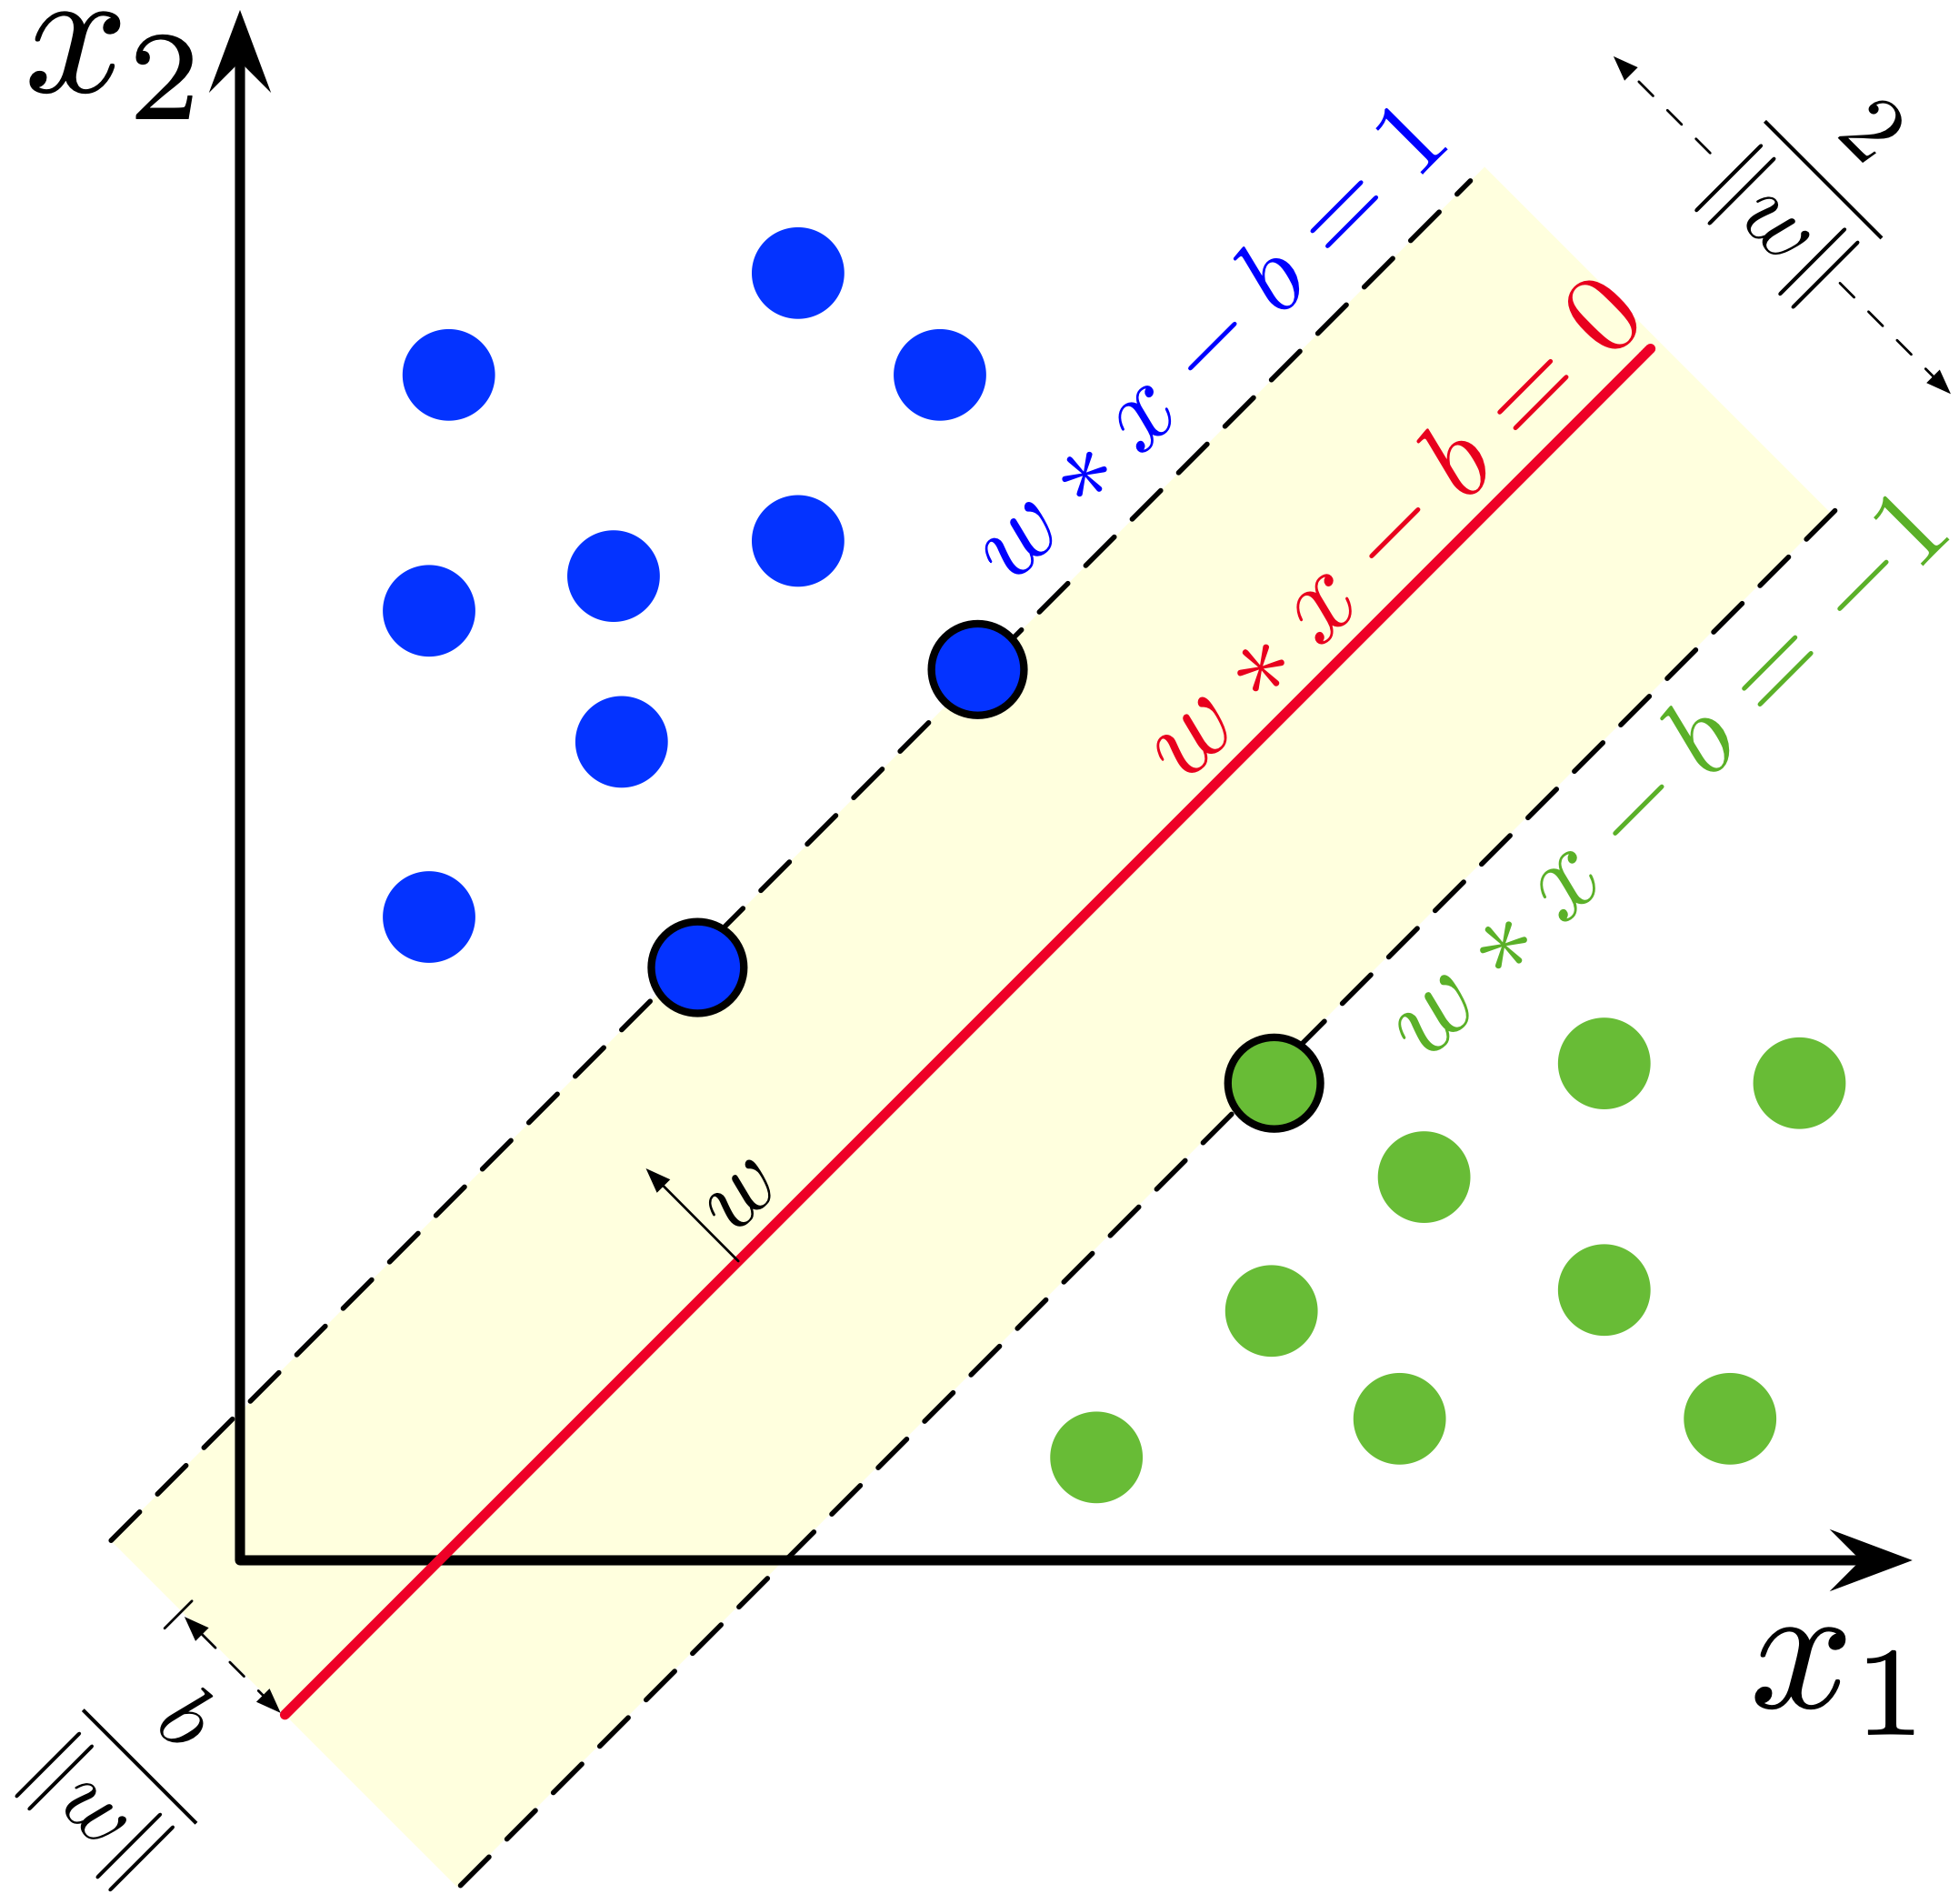
\includegraphics[width=0.6\textwidth]{figures/svm_margin.png}
    \caption{Margins and decision boundary.}
    \label{fig:svm_margin}
\end{figure}

\subsubsection{Finding $\vec{\beta}$ and $\beta_0$ specifying the maximum-margin hyperplane}
\subsubsubsection{Formulating the optimization problem}
From figure \ref{fig:dist_p_h} we the that the distance between a point $\vec{x}^*$ and
a hyperplane $g(\vec{x}) = \vec{w}^T - b = 0$ is given by
\begin{equation}
    \text{distance} = \left| \frac{\vec{w}^T\vec{x}^*}{||\vec{w}||} - \frac{b}{||\vec{w}||} \right| = \frac{|g(x^*)|}{||\vec{w}||}
\end{equation}
($\vec{w} = \vec{\beta}$, $b = -\beta_0$).

\begin{figure}[!htb]
    \centering
    \includesvg[width=0.6\textwidth]{figures/distance_p_h.svg}
    \caption{Distance between a point and a hyperplane.}
    \label{fig:dist_p_h}
\end{figure}

Therefore, maximizing the minimum distance to any point in $\mathcal{D} = \{ \vec{x}_i, c_i \}$ is equivalent to

\begin{equation}
    \label{eq:svm_optimization_problem}
    \vec{\beta}, \beta_0=\underset{\vec{\beta}, \beta_0}{\operatorname{argmax}}\left\{\min _i \frac{c_i \cdot\left(\vec{x}_i^T \vec{\beta}+\beta_0\right)}{\|\vec{\beta}\|}\right\}
\end{equation}

where $c_i g(\vec{x}_i) = |g(\vec{x}_i)|$ for correct classification by the decision function, which we require.

\subsubsubsection{Reformulating into constraint minimization}
Any change in magnitude of $\vec{\beta}$ can be compensated by a change in $\beta_0$
with regards to the decision function. We therefore set
\begin{equation}
    c_0 \cdot (\vec{x}_0^T \vec{\beta} + \beta_0) = 1 \text{ for the closest point } \vec{x}_0 \text{ to the hyperplane}
\end{equation}
without loss of generality, also defining the margins as $g(\vec{x}) = \pm 1$. From this
we follow the constraint
\begin{equation}
    \forall i: c_i \cdot (\vec{x}_i^T \vec{\beta} + \beta_0) \geq 1
\end{equation}
so equation \ref{eq:svm_optimization_problem} can be turned into minimizing $||\vec{\beta}||$,
under the above constraint

\begin{equation}
    \vec{\beta}, \beta_0 = \argmin_{\vec{\beta}, \beta_0} \frac{1}{2} ||\vec{\beta}||^2 \text{ s.t. } c_i \cdot (\vec{x}_i^T \vec{\beta} + \beta_0) \geq 1, \forall i \in \{1, \ldots, N\}
\end{equation}

which is called the \textbf{primal problem}.

\greenbox{This problem can be solved with a standard quadratic programming solver.}

\problem{This primal problem scales mostly with the dimensionality of the feature
matrix, which will be very large, when we later go to kernelized SVMs, which we do as
in high-dimensions classes tend to become linearly separable.}

\greenbox{By going from the \textit{primal} to the \textit{dual problem},
we can go from a problem scaling mostly with the dimensionality of the feature
matrix to one scaling mostly with the number of data points. This makes problems
with huge numbers of data points difficult, but shines for moderate
amounts of data but huge feature vectors.}


\subsubsubsection{Intermezzo: Primal and Dual Problems in Quadratic Programming\skipthis}
Consider the general problem (\textit{primal problem})
\begin{equation}
    \vec{\beta}^* = \argmin f(\vec{\beta}) \text{ s.t. } g_j(\vec{\beta}) \leq 0, h_k(\vec{\beta}) = 0
\end{equation}
where $f(\vec{\beta})$ is quadratic in $\vec{\beta}$, and $g_j(\vec{\beta})$ and $h_k(\vec{\beta})$ are affine in $\vec{\beta}$ (linear plus constant).
$g_j$ and $h_k$ are the \textit{inequality} and \textit{equality constraints}.
\bluebox{Every \textit{primal problem} has a \textit{dual problem}.}
We get from the primal to the dual problem, by writing the Lagrangian
\begin{equation}
    \mathcal{L}(\vec{\beta}, \vec{\alpha}, \vec{\lambda}) = f(\vec{\beta}) + \sum_j \alpha_j g_j(\vec{\beta}) + \sum_k \lambda_k h_k(\vec{\beta})
\end{equation}
and by using the conditions for the extremum
\begin{equation}
    \partial_{\beta_i} \mathcal{L} = 0, \quad \partial_{\lambda_k} \mathcal{L} = 0
\end{equation}
to eliminate $\vec{\beta}$ from the Lagrangian, yielding the 
reduced Lagrangian $\mathcal{L}( \vec{\alpha}, \vec{\lambda})$.

By \textit{strong duality} and the \textit{Karush-Kuhn-Tucker conditions}, the solution of the dual problem

\begin{equation}
    \vec{\alpha}^* = \argmax \mathcal{L}(\vec{\alpha}, \vec{\lambda}), \quad \text{s.t. } \alpha_j \geq 0
\end{equation}

is the same as the solution of the primal problem.

\subsubsubsection{Reformulating into a dual problem}

We can write the minimization in terms of a Lagrangian

\begin{equation}
    \mathcal{L}(\vec{\beta}, \beta_0, \vec{\alpha}) = \frac{1}{2} \vec{\beta}^T \vec{\beta} - \sum_{i=1}^N \alpha_i \left[ c_i \left( \vec{x}_i^T \vec{\beta} + \beta_0 \right) - 1 \right]
\end{equation}

with \textit{Lagrange multipliers} $\alpha_i$.

By using
\begin{equation}
    \begin{gathered}
    \frac{\partial \mathcal{L}}{\partial \vec{\beta}}=0 \rightarrow \hat{\beta}=\sum_{i=1}^N \alpha_i c_i \vec{x}_i \\
    \frac{\partial \mathcal{L}}{\partial \beta_0}=0 \rightarrow \sum_{i=1}^N \alpha_i c_i=0
    \end{gathered}
\end{equation}
with this we can simplify the Lagrangian

\begin{equation}
    \begin{aligned}
    \mathcal{L}(\vec{\beta}, \beta_0, \vec{\alpha}) &= \frac{1}{2} \vec{\beta}^T \vec{\beta} - \sum_{i=1}^N \alpha_i \left[ c_i \left( \vec{x}_i^T \vec{\beta} + \beta_0 \right) - 1 \right] \\
                                                    &= \frac{1}{2} \vec{\beta}^T \vec{\beta} - \underbrace{\left(\sum_{i=1}^N \alpha_i c_i \vec{x}_i^T\right)}_{=\vec{\beta}^T} \vec{\beta} - \beta_0 \underbrace{\sum_{i=1}^N \alpha_i c_i}_{=0} + \sum_{i=1}^N \alpha_i  \\
                                                    &= - \frac{1}{2} \vec{\beta}^T \vec{\beta} + \sum_{i=1}^N \alpha_i
    \end{aligned}
\end{equation}

and finally eliminate $\vec{\beta}$, yielding the \textit{dual problem}.

\begin{equation}
    \vec{\alpha}^* = \argmax_{\vec{\alpha}} \left\{ -\frac{1}{2} \norm{\sum_{i=1}^N \alpha_i c_i \vec{x}_i}^2 + \sum_{i=1}^N \alpha_i \right\} \text{ s.t. } \alpha_i \geq 0, \sum_{i=1}^N \alpha_i c_i = 0
\end{equation}

We can rewrite this to

\begin{equation}
    \vec{\alpha}^* = \argmin_{\vec{\alpha}} \frac{1}{2} \vec{\alpha} \operatorname{diag}(\vec{c}) \underbrace{\mat{X} \mat{X}^T}_{=:G \in \mathbb{R}^{N\times N}} \operatorname{diag}(\vec{c}) \vec{\alpha} - \vec{1}^T \vec{\alpha} \text{ s.t. } \vec{\alpha} \geq 0, \vec{c}^T \vec{\alpha} = 0
\end{equation}

\greenbox{So we have turned a problem of finding $\vec{\beta} \in \mathbb{R}^p$ into a problem of finding $\vec{\alpha} \in \mathbb{R}^N$.}

\greenbox{Here the data occurs only in form of the Gram matrix $G = \mat{X} \mat{X}^T$, which is a $N \times N$ matrix,
so the scaling of the problem is benevolent for large feature vectors (large $p$)}

Having obtained the optimal $\vec{\alpha}^*$ the decision function is

\begin{equation}
    g(\vec{x}) = \vec{\beta}^T \vec{x} + \beta_0 = \sum_{i=1}^N \alpha_i^* c_i \vec{x}_i^T \vec{x} + \beta_0
\end{equation}

\greenbox{So also in the decision function, we only need scalar products $\vec{x}_i^T \vec{x}$, which are later
replaced by kernel functions (the same goes for the entries of the Gram matrix) - allowing for non-linear decision boundaries (separation in theoretically
infinitely expanded feature space). And for the decision we only need $\vec{\alpha}^* \in \mathbb{R}^N$ and $\beta_0$
not $\vec{\beta} \in \mathbb{R}^p$, which is problematic for large $p$.}

\subsubsection{Relaxing the constraint of linear separability - soft-margin SVM}
\idea{Add a regularization to the loss penalizing points crossing the margin (not the decision boundary),
depending on how far they have strayed off from their correct side.}

We use the penalty (\textit{slack variable})
\begin{equation}
    \xi_i = \begin{cases}
        \text{point on the correct side of the margin} & \xi_i = 0 \\
        \text{point on the wrong side of the margin} & \xi_i = |c_i - g(\vec{x}_i)|
    \end{cases} \geq 0 \forall i
\end{equation}

\pinkbox{\textbf{What are the support vectors in the relaxed case?}: Now the points on the wrong side of the margin 
are also support vectors. Generally support vectors are those that have an influence 
on the location of the decision boundary. Note that SVM is not a probability model, 
we just draw a boundary. The support vectors are those where when we would leave away 
all other vectors in the data set we would still retain the same optimal boundary (which 
can of course be described by less parameters than by the support vectors).}

A soft margin is illustrated in figure \ref{fig:soft_margin}.

\begin{figure}[!htb]
    \centering
    \includesvg[width=0.9\textwidth]{figures/soft_svm.svg}
    \caption{Soft margin.}
    \label{fig:soft_margin}
\end{figure}

The new optimization problem is

\begin{equation}
    \begin{gathered}
        \vec{\beta}, \beta_0=\underset{\vec{\beta}, \beta_0}{\operatorname{argmin}}\left\{\frac{1}{2}\|\vec{\beta}\|^2-\sum_{i=1}^N \alpha_i\left[c_i \cdot\left(\vec{x}_i^T \vec{\beta}+\beta_0\right)-1\right]+\gamma \sum_{i=1}^N \xi_i-\sum_{i=1}^N \lambda_i \xi_i\right\} \\
        \text{s.t. } c_i \cdot\left(\vec{x}_i^T \vec{\beta}+\beta_0\right) \geq 1-\xi_i, \quad \xi_i \geq 0, \quad \lambda_i \geq 0
    \end{gathered}
\end{equation}

where $\gamma$ regulates the strength of the penalty.

\yellowbox{\textbf{Note on $\gamma$}: Dividing by $\gamma$, we can interpret this as a regularization on $||\vec{\beta}||^2$.
\begin{itemize}
    \item for large $\gamma$, we have less misclassification, but a smaller margin, as the margin is $\frac{1}{||\vec{\beta}||}$,
    and larger $\gamma$ can be interpreted as a smaller regularization on $||\vec{\beta}||^2$
    \item for small $\gamma$, we have a larger margin, but more misclassification errors
\end{itemize}
This is illustrated in table \ref{tab:svm_gamma}. \textbf{The stronger the regularization $\gamma$, the smaller the number of support vectors.}
As expected the more we penalize points on the wrong side of the margin, 
the closer the margins (less soft) and the less support vectors, so points 
influencing the position of the margin, we have.
}

% table with three graphics for different gamma
\begin{table}[H]
    \centering
    \begin{tabular}{c|c|c}
        \includesvg[width=0.3\textwidth]{figures/soft_svm_gamma_small.svg} & \includesvg[width=0.3\textwidth]{figures/soft_svm_gamma_medium.svg} & \includesvg[width=0.3\textwidth]{figures/soft_svm_gamma_large.svg} \\
        $\gamma$ small & $\gamma$ medium & $\gamma$ large
    \end{tabular}
    \caption{Effect of $\gamma$ ($C$ in the figures) on the soft margin.}
    \label{tab:svm_gamma}
\end{table}

\subsubsection{Kernelized SVM}

\idea{By basis expansion - projection into a higher dimensional feature space - we can make a problem that is not linearly separable linearly separable,
as illustrated in figure \ref{fig:projection_trick}.}

\begin{figure}[!htb]
    \centering
    \includesvg[width=0.8\textwidth]{figures/projection_trick.svg}
    \caption{Projection trick.}
    \label{fig:projection_trick}
\end{figure}

\bluebox{In a space with sufficiently high dimensionality, arbitrary complex patterns are very likely to be linearly separable
(Cover's Function Couting theorem).}

We exapnd into a higher dimensional feature space by

\begin{equation}
    \vec{\phi} : \mathbb{R}^p \rightarrow \mathbb{R}^q, \quad q > p
\end{equation}

for instance

\begin{equation}
    \vec{\phi}(\vec{x}) = \begin{pmatrix}
    x_{i1} \\ \vdots \\ x_{ip} \\ x_{i1}^2 \\ x_{i1}x_{i2} \\ \vdots \\ x_{i(p-1)}x_{ip} \\ x_{ip}^2
    \end{pmatrix}
\end{equation}

\subsubsubsection{Kernel trick for high-D computations}
Let us replace the scalar product in the high dimensional feature space by a kernel function
\begin{equation}
    k(\vec{x}_i, \vec{x}_j) = \vec{\phi}(\vec{x}_i)^T \vec{\phi}(\vec{x}_j)
\end{equation}
which operates on the vectors in the original features space.

\paragraph*{Example: Kernel for polynomial basis expansion}
For instance
\begin{equation}
    k(\vec{x}_i, \vec{x}_j) = (1 + \vec{x}_i^T \vec{x}_j)^d
\end{equation}
based on the low-dimensional scalar product $\vec{x}_i^T \vec{x}_j$ is equivalent to a 
polynomial basis expansion of degree $d$. For $d = 2$ this corresponts to the
feature expansion

\begin{equation}
    \vec{\phi}(\vec{x}) = \begin{pmatrix}
    1 \\ \sqrt{2} x_1 \\ \sqrt{2} x_2 \\ x_1^2 \\ x_2^2 \\ \sqrt{2} x_1 x_2
    \end{pmatrix}
\end{equation}

\paragraph*{Further Kernels: Sigmoid and Gaussian RBF}
\begin{itemize}
    \item \textbf{Sigmoid kernel:} $k(\vec{x}_i, \vec{x}_j) = \tanh(\kappa \vec{x}_i^T \vec{x}_j + \theta)$, parameters $\kappa, \theta$
    \item \textbf{Gaussian RBF kernel:} $k(\vec{x}_i, \vec{x}_j) = \exp\left(-\frac{||\vec{x}_i - \vec{x}_j||^2}{2\sigma^2}\right)$, parameter $\sigma$
\end{itemize}
The Gaussian Kernel is a similarity measure projecting 
into an infinite-dimensional space of all polynomial kernels 
of degrees $p \geq 0$ (which we can see from Taylor 
expanding the Gaussian).

In figure \ref{fig:kernel_trick} we see the effect of different kernels in SVMs.

\begin{figure}

    \centering
    \begin{subfigure}{0.45\textwidth}
      \centering
      \includesvg[width=.95\linewidth]{figures/poly_kernel.svg}
      \caption{SVM with polynomial kernel.}
      \label{fig:poly_kernel}
    \end{subfigure}%



    \begin{subfigure}{0.45\textwidth}
      \centering
      \includesvg[width=.95\linewidth]{figures/rbf_kernel.svg}
      \caption{SVM with RBF kernel.}
      \label{fig:rbf_kernel}
    \end{subfigure}



    \begin{subfigure}{0.45\textwidth}
        \centering
        \includesvg[width=.95\linewidth]{figures/sigmoid_kernel.svg}
        \caption{SVM with sigmoid kernel.}
        \label{fig:sigmoid_kernel}
      \end{subfigure}

    \caption{Effect of different kernels in SVMs.}
    \label{fig:kernel_trick}

\end{figure}

\subsubsubsection{Kernel SVM is where the dual formulation shines}
For Kernelized SVMs, in the dual formulation
\begin{equation}
    \vec{\alpha}^* = \argmin_{\vec{\alpha}} \frac{1}{2} \vec{\alpha} \operatorname{diag}(\vec{c}) \underbrace{\mat{X} \mat{X}^T}_{=:G \in \mathbb{R}^{N\times N}} \operatorname{diag}(\vec{c}) \vec{\alpha} - \vec{1}^T \vec{\alpha} \text{ s.t. } \vec{\alpha} \geq 0, \vec{c}^T \vec{\alpha} = 0
\end{equation}
the Gram matrix changes to
\begin{equation}
    \mat{G} = \mat{\Phi} \mat{\Phi}^T, \quad G_{ij} = k(\vec{x}_i, \vec{x}_j)
\end{equation}
where we need $N\times N$ applications of the kernel function $k$.

Classification of a new point $\vec{x}$ is done by
\begin{equation}
    g(\vec{x}) = \sum_{i=1}^N \alpha_i^* c_i k(\vec{x}_i, \vec{x}) + \beta_0, \quad N \text{ samples in training set}
\end{equation}

\subsubsection{Multiclass SVM}
A simple option is to train a 1-vs-all classifier for all classes and then use
\begin{equation}
    \hat{c} = \argmax_k g_k(\vec{x}), \quad g_k(\vec{x}) = \vec{\beta}_k^T \vec{x} + \beta_{0k}
\end{equation}

\note{\enquote{but it cannot capture correlations between the different classes since 
it breaks a multiclass problem into multiple independent binary problems.}
There are also approaches using multi-class objective functions \citep{crammer01}.}

\greenbox{So everything just depends on the kernel and we can go to effectively infinite dimensions by a kernel function.
\textbf{The dual formulation enables kernelization}.}

\subsection{K-Nearest Neighbor classifier}
kNN is a non-parametric, algorithmic modeling approach, where a new point
\begin{itemize}
    \item kNN-regression: is assigned the average of the $k$ nearest neighbors
    \item kNN-classification: is assigned a class by majority vote of the $k$ nearest neighbors
\end{itemize}
There is \textcolor{green1}{no training needed} but the \textcolor{red1}{model is the training data itself (so the model is possibly very large)}.

In classification, the probability of class $l$ at a point $\vec{x}_0$ is given by

\begin{equation}
    \hat{p}(c_0 = l|\vec{x}_0) = \frac{\# \text{nearest neighbors of class l}}{k} = \frac{|\{ \vec{x}_i \in l \cap H_k(\vec{x}_0) \}|}{|\{ \vec{x}_i \in H_k(\vec{x}_0) \}|}
\end{equation}

A weighted approach with closer neighbors having more influence is also possible.

\subsubsection{Dependence of the classification on $k$ - balance between over- and underfitting}
We note
\begin{itemize}
    \item \textbf{Small $k$:} more flexible, but more sensitive to noise (for $k=1$ Delauney triangulation, so Vornoi cells)
    \item \textbf{Large $k$:} less flexible, but more robust to noise
\end{itemize}
which is illustrated in table \ref{tab:knn_k}.

% two fields, one small k, one large k
\begin{table}[H]
    \centering
    \begin{tabular}{c|c}
        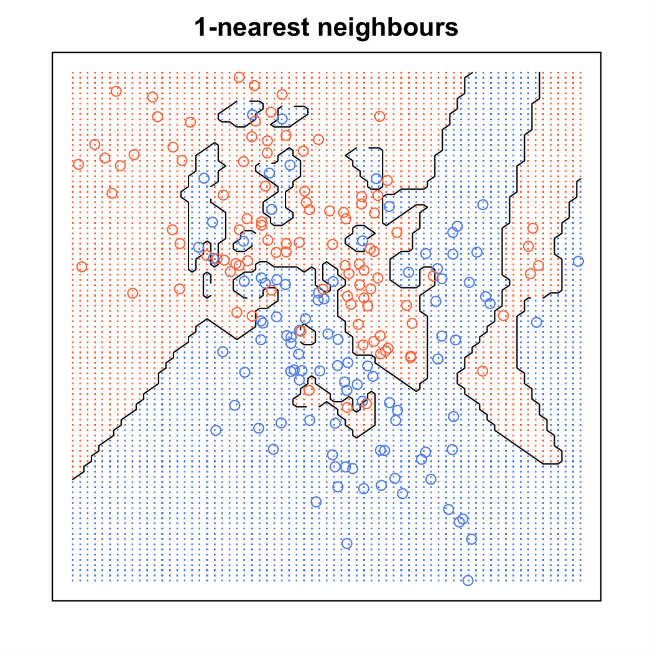
\includegraphics[width=0.45\textwidth]{figures/knn_small_k.png} & 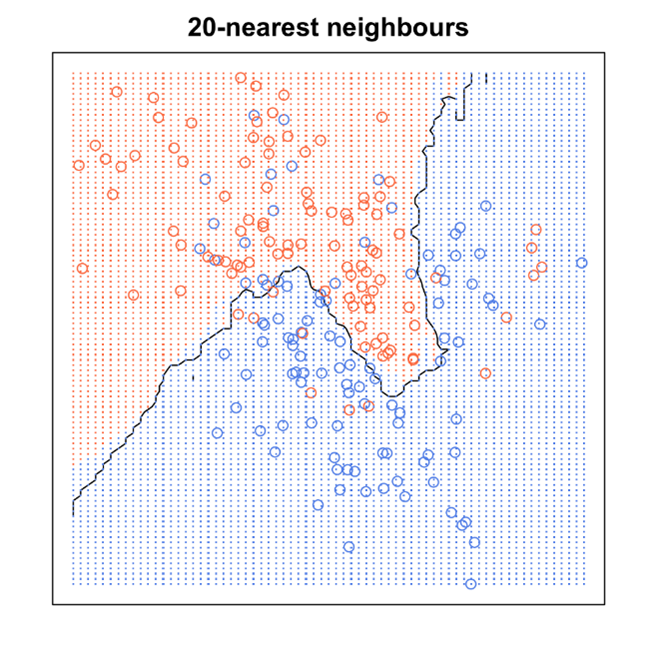
\includegraphics[width=0.45\textwidth]{figures/knn_large_k.png} \\
        Small $k$ & Large $k$
    \end{tabular}
    \caption{Effect of $k$ on kNN.}
    \label{tab:knn_k}
\end{table}

\pinkbox{\textbf{Number of effective parameters:} While kNN is non-parametric,
so there is no fixed number of parameters learned independent of the size of the
training set, there are effectively $\sim \frac{k}{N}$ neighborhoods where one
parameter - the class - is learned.}

\subsubsection{Advantages and Disadvantages of kNN}
\begin{itemize}
    \item \textcolor{green1}{Advantages:} can approximate any distribution, fast training (only store the data)
    \item \textcolor{red1}{Disadvantages:}
    \begin{itemize}
        \item entire data-set is stored (large model); \textcolor{green1}{use e.g. Hart condensing to reduce the data set while keeping the decision boundary}
    \end{itemize}
\end{itemize}

\subsection{Logistic classification}

We have a data set $\mathcal{D} = \{ \vec{x}_i, c_i \}$, $c_i \in \{0, 1\}$, and we want to model the probability of class $1$ at a new point $\vec{x}$.

\subsubsection{GLM perspective on logistic regression}
At every point $\vec{x}$, we model the class probability by a Bernoulli distribution
\begin{equation}
    p(c | \vec{x}) = \begin{cases}
        1- \mu(\vec{x}) & c = 0 \\
        \mu(\vec{x}) & c = 1
    \end{cases}
\end{equation}
where the model of $\mu(\vec{x})$ is given by the sigmoid
\begin{equation}
    g^{-1}(\eta) = \mu = \sigma(\eta) = \frac{1}{1 + \exp(-\eta)}, \quad \eta = \vec{\beta}^T \vec{x}
\end{equation}
which in the GLM framework can be followed from the finding the canonical link function. For 1D data,
this is illustrated in figure \ref{fig:logistic_regression}.

\begin{figure}[!htb]
    \centering
    \includesvg[width=0.6\textwidth]{figures/log_reg.svg}
    \caption{Logistic regression.}
    \label{fig:logistic_regression}
\end{figure}

\note{Here we assume $\vec{x}$ to have a constant $1$ as first entry, allowing for an offset $\beta_0$.}

The link function is given by
\begin{equation}
    g(\mu) = \eta = \vec{\beta}^T \vec{x} = \log \frac{\mu}{1-\mu}
\end{equation}
\bluebox{So the logarithmic odds
\begin{equation}
    \text{odds} = \frac{\text{probability that outcome occurs}}{\text{probability that outcome does not occur}} = \frac{\mu}{1-\mu}
\end{equation}
are a linear function of the independent variables.
}

\greenbox{For $\vec{x} \in \mathbb{R}^p$, we have $\vec{\beta} \in \mathbb{R}^{p}$, so as many parameters to learn as features.
Fitting a multidimensional normal to each class would generally be quadratic in $p$ as of the covariance matrix.}

Our decision rule is
\begin{equation}
    \begin{aligned}
        \hat{c} &= \argmax_c p(c | \vec{x}; \vec{\beta}) \\
        &= \begin{cases}
            1 & \mu(\vec{x}) \geq 0.5 \\
            0 & \mu(\vec{x}) < 0.5
        \end{cases} \\
        &= \begin{cases}
            1 & \log \frac{\mu(\vec{x})}{1-\mu(\vec{x})} \geq 0 \\
            0 & \log \frac{\mu(\vec{x})}{1-\mu(\vec{x})} < 0
        \end{cases} \\
        &= \begin{cases}
            1 & \vec{\beta}^T \vec{x} \geq 0 \\
            0 & \vec{\beta}^T \vec{x} < 0
        \end{cases}
    \end{aligned}
\end{equation}

\subsubsection{Linear classifier perspective on logistic regression}
Let us start by modeling the likelihood with a heaviside function
$p(c = 1|\vec{x}) = \theta(g(\vec{x})) \in \{0,1\}$, $g(\vec{x}) = \vec{w}^T \vec{x} - b$, where
\begin{equation}
    \theta(z) = \begin{cases}
        1 & z \geq 0 \\
        0 & z < 0
    \end{cases}
\end{equation}
This is illustrated in figure \ref{fig:heaviside_classifier}.
\begin{figure}[!htb]
    \centering
    \includesvg[width=0.6\textwidth]{figures/heaviside_classifier.svg}
    \caption{Heaviside classifier.}
    \label{fig:heaviside_classifier}
\end{figure}
\problem{We cannot use the heaviside as a likelihood model, because
there it does not differentiate between different boundaries
separating the data.}
\idea{Use the sigmoid $p(c = 1|\vec{x}) = \sigma(g(\vec{x}))$ as a likelihood model.
Where $||\vec{w}||$ gives how fast the decision transitions
from $0$ to $1$ and $\frac{b}{||w||}$ gives the offset of the decision
plane along $\vec{w}$. For $||\vec{w}|| \rightarrow \infty$ we have 
a step function again.}

A sigmoid model for the likelihood is illustrated in figure \ref{fig:sigmoid_classifier}.

\begin{figure}

    \centering
    \begin{subfigure}{0.55\textwidth}
      \centering
      \includesvg[width=.95\linewidth]{figures/sigm1.svg}
      \caption{Sigmoid classifier with small $||\vec{w}||$.}
      \label{fig:sigmoid_classifier_small}
    \end{subfigure}%

    \begin{subfigure}{0.55\textwidth}
        \centering
        \includesvg[width=.95\linewidth]{figures/sigm2.svg}
        \caption{Sigmoid classifier with large $||\vec{w}||$.}
        \label{fig:sigmoid_classifier_large}
      \end{subfigure}

    \caption{Sigmoid classifier.}
    \label{fig:sigmoid_classifier}

\end{figure}

\subsubsection{Finding the parameters of $\mu(\vec{x})$, $\vec{\beta}$ by MLE}
The likelihood of a single data point is given by
\begin{equation}
    p(c_i | \vec{x}_i) = (1 - \sigma(\vec{\beta}^T \vec{x}_i))^{1 - c_i} \sigma(\vec{\beta}^T \vec{x}_i)^{c_i}
\end{equation}
As usual, we minimize the negative log-likelihood
\begin{equation}
    \begin{aligned}
        \vec{\hat{\beta}}, \hat{\beta}_0 &= \argmin_{\vec{\beta}, \beta_0} \sum_{i=1}^N -\log(p(c_i | \vec{x}_i)) \\
        &=\sum_{i=1}^N-c_i \log \sigma\left(\vec{\beta}^T \vec{x}_i\right)-\left(1-c_i\right) \log \left(1-\sigma\left(\vec{\beta}^T \vec{x}_i\right)\right) \\
        &=-\sum_{i=1}^N \left( c_i \vec{\beta}^T \vec{x}_i - \log(1 + \exp(\vec{\beta}^T \vec{x}_i)) \right)
    \end{aligned}
\end{equation}
which is called \textcolor{blue1}{logistic loss} or \textcolor{blue1}{cross-entropy loss} or 
\textcolor{blue1}{log-loss} which is concave, \textbf{so we use Newton-Raphson to find the minimum}
(there is no closed-form solution).

\subsubsubsection{Understanding the terms in the negative log-loss as penalties}
For a single data-point, the negative log-loss given $\mu$
and the true class $c$ is illustrated in figure \ref{fig:log_loss}.
Predicting $\mu > 0.5$ when the true class is $0$ comes
with an increasingly high penalty.

\begin{figure}[!htb]
    \centering
    \includesvg[width=0.6\textwidth]{figures/log_loss.svg}
    \caption{Negative log-loss for a single data point.}
    \label{fig:log_loss}
\end{figure}

\subsubsubsection{For linearly separable data, $||\vec{\beta}|| \rightarrow \infty$ minimizes the loss}
For linearly separable data
\begin{equation}
    c_i = 1 \rightarrow \vec{\beta}^T \vec{x} \geq 0, \quad y_i = 0 \rightarrow \vec{\beta}^T \vec{x} < 0
\end{equation}
is possible. Then $||\vec{\beta}|| \rightarrow \infty$ minimizes the
loss for any $\vec{x}$ (we can also see this from the original
loss as of $\sigma(\vec{\beta}^T \vec{x}) \rightarrow \theta(\vec{\beta}^T \vec{x})$ for $||\vec{w}|| \rightarrow \infty$).

\bluebox{\textbf{Intuition}: In the large $||\vec{\beta}||$ limit, different classifiers are not distinguishable
anymore by the likelihood, as illustrated in figure \ref{fig:separable_w_inf}.}

\begin{figure}[!htb]
    \centering
    \includesvg[width=0.75\textwidth]{figures/separable_w_inf.svg}
    \caption{Large $||\vec{\beta}||$ limit for linearly separable data.}
    \label{fig:separable_w_inf}
\end{figure}

\note{For data that is not linearly separable, $||\vec{\beta}|| \rightarrow \infty$ leads to divergent
error terms so is not optimal, so $||\vec{\beta}|| \rightarrow \infty$ is not optimal, see
figure \ref{fig:non_separable_w_inf}.}

\begin{figure}[!htb]
    \centering
    \includesvg[width=0.75\textwidth]{figures/non_separable_w_inf.svg}
    \caption{Large $||\vec{\beta}||$ limit for non-linearly separable data.}
    \label{fig:non_separable_w_inf}
\end{figure}

\subsubsubsection{The decision boundary in logistic regression is linear}
The decision boundary is at $\mu = \frac{1}{2}$, so
\begin{equation}
    \vec{\beta}^T \vec{x} = \log \frac{\mu}{1-\mu} = 0
\end{equation}

\subsubsection{Multinomial Logistic Regression}
Consider multiclass data $\mathcal{D} = \{ \vec{x}_i, c_i \}$, $c_i \in \{1, \ldots, K\}$, and we want to model the probability of class $k$ at a new point $\vec{x}$.
\bluebox{We directly model the class probabilities, the parameters of a categorical model, by a soft(arg)max function.
We do not make assumptions on the distribution of the features (like a Gaussian, as done in discriminant analysis).}

\subsubsubsection{Perspective of a multicategorical probability model}
Our probability model for obtaining class $c_i = k$ at a point $\vec{x}_i$ is given by the multicategorical
\begin{equation}
    p\left(c_i = k | \vec{x}_i; \{\mu_{\ell} \}_{\ell=1}^K\right) = \mu_k(\vec{x}_i), \quad \sum_{k=1}^K \mu_k(\vec{x}_i) = 1
\end{equation}
which if $\vec{k}$ is the $1$-hot encoding of $k$ is given by
\begin{equation}
    p\left(c_i = \vec{k} | \vec{x}_i; \{\mu_{\ell} \}_{\ell=1}^K\right) = \prod_{j=1}^K \mu_j(\vec{x}_i)^{k_j}
\end{equation}
where again, we model the parameters of our probability model $p_k = \mu_k$ as a function of the features $\vec{x}$.

\note{This is a different perspective than discriminant analysis. There we assume that given the class,
the features are brought forth by a given distribution and from Bayes' theorem we can get class probabilities 
at a given location. Here we assume the $\vec{x}_i$ to be fixed and directly model the likelihood of the given
class probabilities under a probabalistic model which mean (/parameters) are a function of the features.}

But what is our model for the class probabilities?

\subsubsubsection{Derivation of the class probabilities | soft(arg)max}
Let our starting point be, that the odds are linear in the parameters,
as in the two-class case, but now with a reference class $K$.
\begin{equation}
    \begin{gathered}
        \text{logistic odds for } \ell<K: \log \frac{p(c_i = \ell | \vec{x}_i)}{p(c_i = K | \vec{x}_i)} = \vec{\beta}_\ell^T \vec{x}_i, \quad \vec{x}_i = \begin{pmatrix}
            1 \\ x_{i1} \\ \vdots \\ x_{ip}
        \end{pmatrix} \\
        \rightarrow p_\ell = \exp(\vec{\beta}_\ell^T \vec{x}_i) \underbrace{p(c_i = K | \vec{x}_i)}_{p_K}
    \end{gathered}
\end{equation}
For the probability of the reference class, we can use
\begin{equation}
    \begin{gathered}
    \sum_{\ell=1}^{K} p_\ell = 1 \quad \rightarrow \quad p_K = 1 - \sum_{\ell=1}^{K-1} p_\ell = 1 - \sum_{\ell=1}^{K-1} \exp(\vec{\beta}_\ell^T \vec{x}_i) p_K \\
    \rightarrow p_K = \left[ 1 + \sum_{\ell=1}^{K-1} \exp(\vec{\beta}_\ell^T \vec{x}_i) \right]^{-1}
    \end{gathered}
\end{equation}
giving us the class probabilities
\begin{equation}
    p_\ell = \frac{\exp(\vec{\beta}_\ell^T \vec{x}_i)}{1 + \sum_{\xi=1}^{K-1} \exp(\vec{\beta}_\xi^T \vec{x}_i)}
\end{equation}
Assume we would apply the same log-odds formula to the reference class,
\begin{equation}
    0 = \log \frac{p(c_i = K | \vec{x}_i)}{p(c_i = K | \vec{x}_i)} = \vec{\beta}_K^T \vec{x}_i
\end{equation}
which always holds only if $\vec{\beta}_K = \vec{0}$. With this we get the
soft(arg)max function
\begin{equation}
    p_\ell = \operatorname{softargmax}\left( \begin{pmatrix}
        \vec{\beta}_1^T \vec{x}_i \\ \vdots \\ \vec{\beta}_{K}^T \vec{x}_i
    \end{pmatrix} \right)_\ell = \frac{\exp(\vec{\beta}_\ell^T \vec{x}_i)}{\sum_{\xi=1}^{K} \exp(\vec{\beta}_\xi^T \vec{x}_i)}
\end{equation}

\subsubsubsection{An engineering style approach to multinomial logistic classification}
Let us start somewhat fresh. 
\bluebox{Given data $\mathcal{D} = \{ \vec{x}_i, c_i \}$, $c_i \in \{1, \ldots, K\}$, for a new
point $\vec{x}$ we want to estimate the class.}
\idea{Use a linear decision function $g_k(\vec{x}) = \vec{\beta}_k^T \vec{x},k=1,\dots,K$ for each class and predict
\begin{equation}
    \hat{c} = \argmax_k g_k(\vec{x}) = \argmax_k \vec{\beta}_k^T \vec{x}
\end{equation}
so if $c$ is given in 1-hot encoding
\begin{equation}
    \hat{c}_k = \begin{cases}
        1 & k = \argmax_k \vec{\beta}_k^T \vec{x} \\
        0 & \text{else}
    \end{cases} \quad \rightarrow \quad \vec{\hat{c}} \in \{0,1\}^K
\end{equation}
}
\yellowbox{Much more than a 1-hot result $\vec{\hat{c}}$, we want a vector of class probabilities $\vec{\mu}(\vec{x})$, which
we get by using the soft(arg)max function instead of the argmax function.}

Let us collect the $\vec{\beta}_k$ in a matrix
\begin{equation}
    \mat{B} = \begin{pmatrix}
        - & \vec{\beta}_1^T & - \\ - & \vdots & - \\ - & \vec{\beta}_K^T & -
    \end{pmatrix}
\end{equation}

then at a point $\vec{x}$, the class probabilities are given by
the model

\begin{equation}
    \label{eq:softargmax}
    \vec{\mu}(\vec{x}) = \operatorname{softargmax}(\mat{B} \vec{x}) = \frac{1}{\sum_{\xi=1}^{K} \exp(\vec{\beta}_\xi^T \vec{x})} \begin{pmatrix}
        \exp(\vec{\beta}_1^T \vec{x}) \\ \vdots \\ \exp(\vec{\beta}_K^T \vec{x})
    \end{pmatrix}
\end{equation}

which are the parameters of our categorical distribution, from which we follow the likelihood of the class labels
given the $\vec{x}_i$ and $\mat{B}$, where $\mat{B}$ can be found by MLE.

The formula \ref{eq:softargmax} can be represented by an engineering style diagram, see figure \ref{fig:softargmax_engineering}.

\begin{figure}[!htb]
    \centering
    \includesvg[width=0.9\textwidth]{figures/softargmax_engineering.svg}
    \caption{Soft(arg)max function in an engineering style diagram.}
    \label{fig:softargmax_engineering}
\end{figure}

\pinkbox{This diagram (fig. \ref{fig:softargmax_engineering}) represents the output layer of a neural network for a classification into $K$ classes.}

\subsubsubsection{Perceptron for binary classification}
Let us go back to the binary case, where we model $p(c = 1 | \vec{x}) = \mu(\vec{x}) = \sigma(\vec{\beta}^T \vec{x})$
by a sigmoid function ($p(c = 0 | \vec{x}) = 1 - \mu(\vec{x})$). This model is illustrated in figure \ref{fig:perceptron}
(with an offset here not by engineering on $\vec{x}$ but a bias term $b$).

\begin{figure}[!htb]
    \centering
    \includesvg[width=0.8\textwidth]{figures/perceptron.svg}
    \caption{Perceptron.}
    \label{fig:perceptron}
\end{figure}

\greenbox{The perceptron is visualizes the logistic regression model for binary classification. It can linearly separate
classes with decision boundary perpendicular to $\vec{\beta}$ and offset $-\frac{b}{||\vec{\beta}||}$ (minted
here $+b$ not $-b$ as previously in the formula).}

\subsection{A primer on neural networks in the context of classification}
\problem{The perceptron can only separate linearly separable data.}
\idea{Use multiple layers to project the data into a higher dimensional space, where it is linearly separable.}

A more complex separation of two classes in 1D is illustrated in figure \ref{fig:nn_1d},
a 2D separation in figure \ref{fig:nn_2d}.

\begin{figure}[!htb]
    \centering
    \includesvg[width=0.8\textwidth]{figures/nn_1d.svg}
    \caption{Complex separation of two classes in 1D.}
    \label{fig:nn_1d}
\end{figure}

\begin{figure}[!htb]
    \centering
    \includesvg[width=0.8\textwidth]{figures/nn_2d.svg}
    \caption{Complex separation of two classes in 2D.}
    \label{fig:nn_2d}
\end{figure}

\pinkbox{\textbf{Example: Multi-Layer perceptron for an XOR Gate}: Consider and XOR with
\begin{equation}
    (x_1,x_2) \in \{-1,1\}^2, \quad \text{unusual convention } -1: \text{true}, 1: \text{false}
\end{equation}
A visualization and perceptron can be found in table \ref{tab:xor_perceptron}.
}

\begin{table}[!htb]
    \centering
    \begin{tabular}{c|c}
        \includesvg[width=0.45\textwidth]{figures/xor.svg} & \includesvg[width=0.45\textwidth]{figures/xor_perceptron.svg} \\
        XOR \textit{classes} & Perceptron
    \end{tabular}
    \caption{XOR and Perceptron.}
    \label{tab:xor_perceptron}
\end{table}

\subsubsection{Neural Network Loss for Classification}
\bluebox{How do we find the weights (and biases) $\vec{W}$ (grouped into
one vector) of a neural network for
the classification of $K$ classes?}

After multiple layers, the output of our neural network are class probabilities
\begin{equation}
    \text{neural network for classification: } \vec{f}_\vec{W}(\vec{x}_i) \in [0,1]^K, \quad \sum_{k=1}^K f_{\vec{W},k}(\vec{x}_i) = 1
\end{equation}
How can we for each data pair $\vec{x}_i, \vec{c}_i$ ($\vec{c}_i$ in $1$-hot encoding) find the error of our prediction?

We use the cross-entropy loss
\begin{equation}
    \epsilon = H(\{\vec{c}_i\}, \{\vec{f}_\vec{W}(\vec{x}_i)\}) = -\sum_{i=1}^N \vec{c}_i^T \log(\vec{f}_\vec{W}(\vec{x}_i))
\end{equation}

\bluebox{\textbf{Neural Network loss in a regression setting:} In the
regression setting}

\subsubsubsection{Intermezzo: Information measures for probability distributions}
The shannon information content $h(x) = \log_2 \frac{1}{p(x)}$ of an event $x$
is a measure of surprise - rare events (low $p(x)$) have high information content,
as they are very surprising. The expected information content is the entropy
\begin{equation}
    H(X) = -\sum_{x \in X} p(x) \log_2 p(x)
\end{equation}
which is high, if we expect a lot of surprise (rare events).
\pinkbox{\textbf{Perspective from information theory:} We would 
like to send a message consisting of the letters $\{A,B,C,D\}=X$. 
Assuming all letters are equally likely, we could let the message 
consist of a sequence of two-bit letters, $A=00,B=01,C=10,D=11$. 
However, we could also encode unambiguously using 
$A=0,B=10,C=110,D=111$ if we assume $P(A) \gg P(B) \gg P(C) \gg P(D)$. 
$H(X)$ then is the number of bits we need on average given 
the probabilities $P(A), P(B), P(C), P(D)$ to encode a 
character.}

\subsubsubsection{Introduction of Cross-Entropy}
Consider for the same feature vectors $\vec{x}_i$ different probabilities $\vec{p}_i$ and $\vec{q}_i$
are assigned. Cross-entropy is a measure of dissimilarity between the two distributions
\begin{equation}
    H(\vec{p}, \vec{q}) = -E_p[\log{q}] =-\sum_{k=1}^K p_k \log(q_k)
\end{equation}
For $p = q$, we get back to the entropy
\begin{equation}
    H(\vec{p}, \vec{p}) = H(\vec{p}) = -E_p[\log{p}] =-\sum_{k=1}^K p_k \log(p_k) = H(\vec{p}) \geq 0 \text{ as } 0 \leq p_k \leq 1
\end{equation}
which by Gibb's inequality
\begin{equation}
    H(\vec{p}, \vec{q}) \geq H(\vec{p}), \quad \text{with equality if and only if } \vec{p} = \vec{q}
\end{equation}
is the minimum of the cross entropy.
\greenbox{The more similar two distributions are, the lower the cross-entropy.}

\subsubsubsection{Relation between cross-entropy and the negative log-likelihood - they're the same}
Consider for a single data point from the training set $\vec{x}_i$, our model
predicts the class probabilities
\begin{equation}
    \vec{\mu} = \vec{f}_\vec{W}(\vec{x}_i) \in [0,1]^K, \quad \sum_{k=1}^K \mu_k = 1
\end{equation}
\problem{We do not have the true distribution of the classes, but only the true class $\vec{c}_i$ in 1-hot encoding.}
\idea{Take $\vec{c}_i$ as a proxy for the true distribution of the classes.}
With this for the class distribution at a single $\vec{x}_i$, the cross-entropy loss is given by
\begin{equation}
    \epsilon_i = H(\vec{c}_i, \vec{\mu}) = -\sum_{k=1}^K c_{ik} \log(\mu_k) = -\log \prod_{k=1}^K \mu_k^{c_{ik}}
\end{equation}
which is just the negative log likelihood at this point. Summing over all data points
we obtain the total loss.

\pagebreak